\documentclass[a4paper,10pt]{article}
\usepackage{geometry}
\geometry{a4paper, portrait, margin=.8in}
\usepackage{amsmath,amsthm,amsfonts,amssymb,bbm,empheq}
\usepackage{paralist,graphics,epsfig,graphicx,epstopdf,mathrsfs}
\usepackage{float,color,ulem,comment,tabulary,cite,booktabs}
\usepackage{multirow,multicol}
\usepackage{epsf,epsfig,subfigure}
\setcounter{MaxMatrixCols}{30}
\usepackage[colorlinks=true]{hyperref}
\hypersetup{urlcolor=blue,linkcolor=black,citecolor=blue,colorlinks=true}
% \usepackage[notref,notcite]{showkeys}
\usepackage{mathpazo}
\usepackage[table,xcdraw]{xcolor}
\usepackage{cite}
\usepackage{svg}

\newcommand{\red}[1]{\textcolor{red}{#1}}
\title{VAE-CME}
\author{Xinyi Zhou}
\date{2023.6.23}

\begin{document}
\tableofcontents
\maketitle

\section{Birth Death Model}
Consider a simple non-Markovian system where molecules are produced at a rate $\rho$ and are removed from the system (degraded) after a fxed time delay $\tau$:
\begin{equation}\label{birth-death}
\emptyset\stackrel{\rho}\rightarrow N, N\stackrel{\tau}\Rightarrow\emptyset
\end{equation}
The training set is the distribution from $1 \times 10^4$ samples using the SSA.In the experiment, we assume $\rho=20$, $\tau=10$ and truncation $N=271$. 

Both encoder and decoder are multilayer perceptron with one hidden layer. The objective function is chosen as the sum of mean-squared-error and KL divergence. For the training we used the standard adaptive moment estimation algorithm (ADAM). The weight of mean-squared-error needs to be increased, and the learning rate needs to be decreased from approximately 0.25 to 0.01 during the training process.

\begin{figure*}[h]
	\centering
	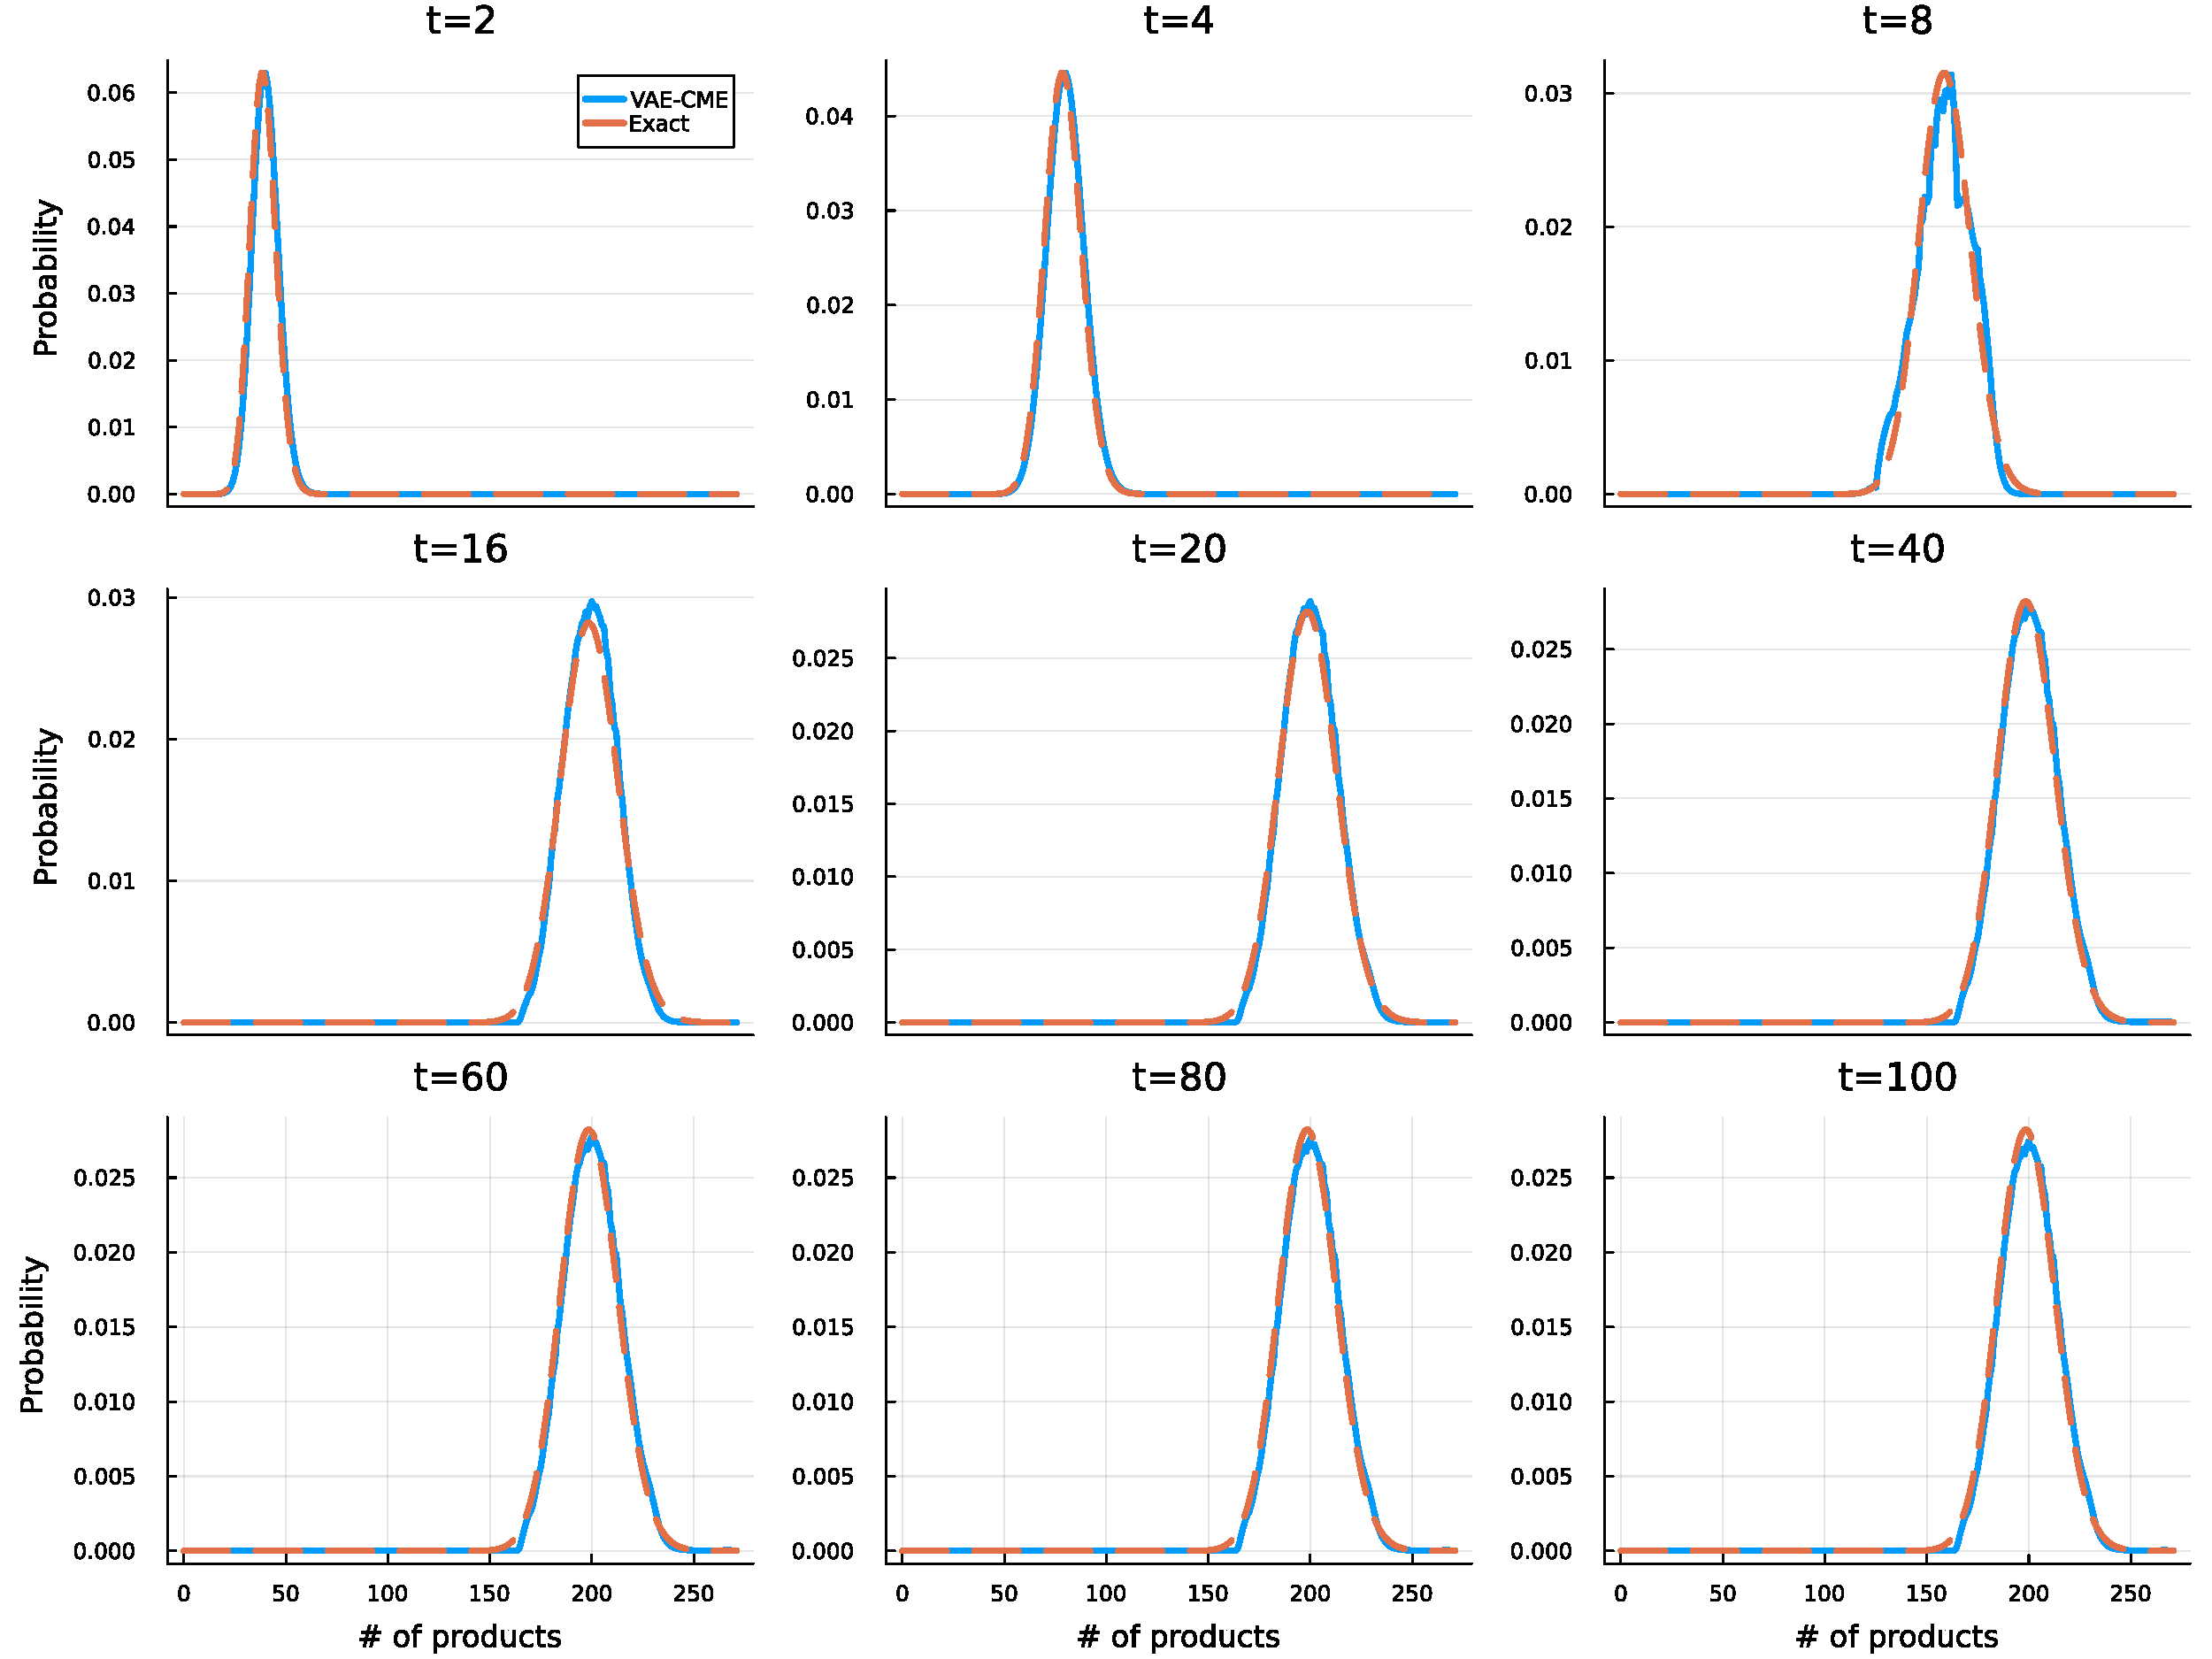
\includegraphics[width=0.75\textwidth]{Figs/Birth_Death_fitting.pdf}
	\caption{Birth Death Model Fitting}\label{Birth Death Model Fitting}  
\end{figure*}

\section{On Off Model}

\section{Bursty Model}

We consider Bursty Model, which is the same as Birth Death Model, except that the binding of RNAPs to the promoter occurs in bursts whose size $i$ is distributed according to the geometric distribution $b^i/(1 + b)^{i+1}$; this can be described by the reaction scheme:
\begin{equation}\label{birth-death}
	\begin{aligned}
		&\emptyset\stackrel{\frac{\alpha\beta^i}{(1+\beta)^{i+1}}}\longrightarrow iN,i=1,2,3,...\\ &N\stackrel{\tau}\Rightarrow\emptyset
	\end{aligned}
\end{equation}
To achieve the best fitting performance, the analytical solution of the Bursty model's probability distribution (See SI in \cite{jiang2021neural}) is used as the training set. In the experiment, we assume $\alpha=0.0282$, $\beta=3.46$, $\tau=120$ and truncation $N=64$.

The same as before, we choose the sum of mean-squared-error and KL divergenc as the  objective  function, ADAM as the optimizer. And the weight of mean-squared-error needs to be increased, the learning rate needs to be decreased
\begin{figure*}[h]
	\centering
	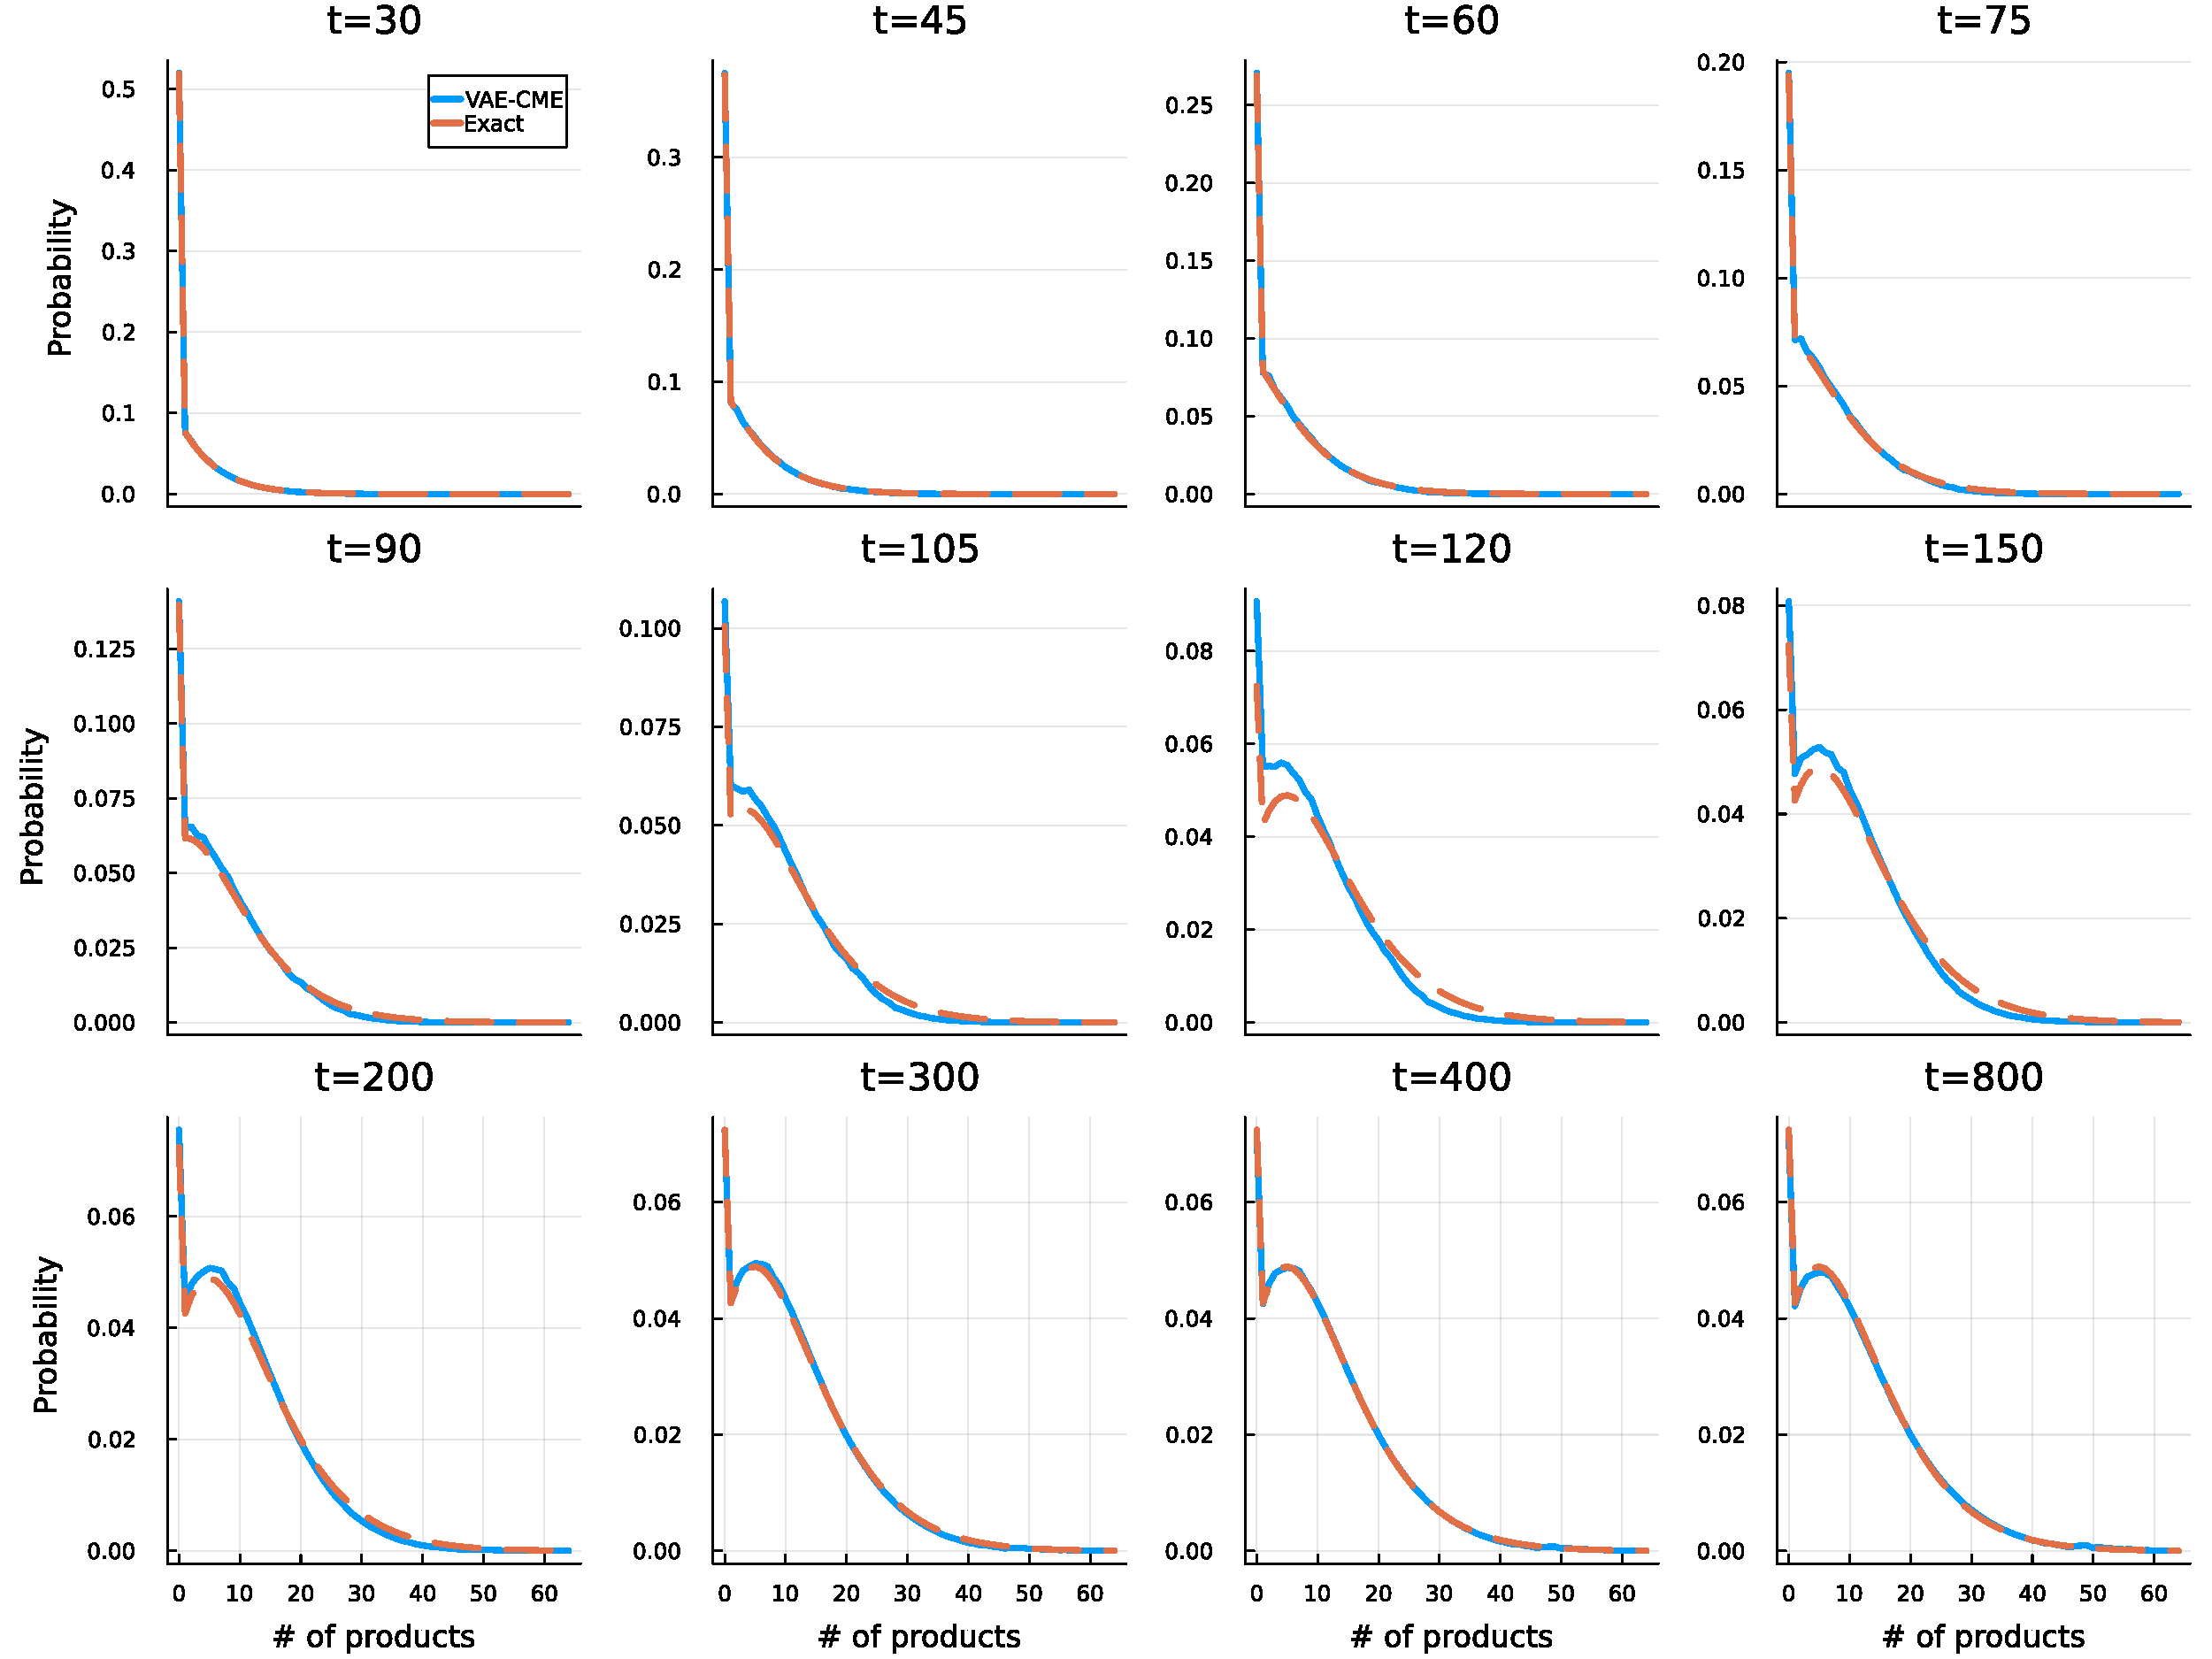
\includegraphics[width=0.75\textwidth]{Figs/Bursty_fitting.pdf}
	\caption{Bursty Model Fitting}\label{Bursty Model Fitting}  
\end{figure*}

\subsection{Control Mean of time delay $\tau$}

\subsection{Control Variance of time delay $\tau$}

\section{Oscillation Model}

\subsection{Reducing sample size}

\section{Exact solution for variable time delay $\tau$}

\bibliographystyle{unsrt}
\bibliography{VAE-CME.bib}
\addcontentsline{toc}{section}{References}

\end{document}